\chapter{Redox activity of Single-azurin at diffferent electrochemical potential}
% !TeX root = ./azurin.tex
\graphicspath{{./chapters/c4_azurin_sm/main/}}
% \externaldocument{./chapters/c4_azurin_sm/si_azurin} 
%%%%%%%%%%%%%%%%%%%%%%%%%%%%%%%%%%%%%%%%%%%%%%%%%%%%%%%%%%%%%%%%%%
%%%%%%% Start the main part of the manuscript here.%%%%%%%%%%%%%%
%%%%%%%%%%%%%%%%%%%%%%%%%%%%%%%%%%%%%%%%%%%%%%%%%%%%%%%%%%%%%%%%%%
\section{Introduction}
Introduction here.
%%%%%%%%%%%%%%----------EXPERIMENTAL SECTION----------%%%%%%%%%%%%%%%%%%%%
\section{Experimental Section}
\subsection{Protein synthesis}
Azurin (wild type) from \textit{Pseudomonas aeruginosa} was expressed in \textit{E. Coli} and purified as described before \citep{kamp1990purification}. BL21 \textit{E.coli} cells were transformed with PGK22 plasmid that carries the gene for azurin. The cells were cultured in Luria Bertani (LB) medium. Then the cells were harvested and resuspended in a 20 \% (w/v) sucrose solution in Tris pH 8 buffer containing $1~\mM$ EDTA. The solution was centrifuged ($8000~$rpm, 20~min) and the supernatant was collected. Copper sulfate was added to the solution for insertion into the active site of azurin. The unwanted proteins were precipitated by addition of concentrated acetic acid until pH 4. The turbid solution was centrifuged at $8000~$rpm for $20~$min. The supernatant was loaded on a CM Sepharose fast flow column and elution was performed in an Akta purifier (GE Healthcare) with a pH gradient from $4$ to $6.9$ in $50~\mM$ ammonium acetate. Fractions containing azurin (inferred from the absorbance at $290~nm and 620~nm$ ) were collected and reduced with sodium dithionite. At this moment the solution contained both zinc and copper azurin. The azurins were purified in a DEAE sepharose column by a salt gradient of 0 to $50~$\mM NaCl in Tris pH8 buffer. Fractions containing copper azurin and zinc azurin were collected and concentrated separately. The purity of the samples was checked by sodium dodecyl sulphate (SDS)-polyacrylamide gel electrophoresis (PAGE) and UV/Vis spectroscopy (Cary 50 spectrophotometer, Varian Inc., Agilent Technologies, USA). The azurins appeared on SDS gel page at $\sim$14 kDa. Both zinc and copper azurin showed a characteristic shoulder at ${\sim}290~\nm$ while Cu azurin showed an additional broad absorption peak at $620~\nm$ when oxidized as can be seen in Figure-S\ref{SIfig: switching}. The ratio $O.D_{628\nm}/O.D_{280\nm}$ for Cu azurin was 0.56 which indicated that all the azurin molecules had a Cu atom. The concentrated protein was stored at $80\degree$ until further use.
\subsection{Fluorescent labeling}
The labeling protocol was based on previous work \cite{nicolardi2012topdown}. ATTO655 NHS-ester was bought from ATTO-TEC GmbH. The buffer containing azurin was replaced with HEPES pH 8.3. ATTO655 was chosen to label the protein because of its stability and light insensitivity in the potential range used for this study. A mixture of $200~\uM$ azurin and ATTO 655 NHS-ester (1:1) was incubated for 45~min. The NHS-ester group reacts with one of the amine group on the protein. The unreacted dyes were removed with a HiTrap desalting column. The labeled protein was concentrated in Tris pH 8.5 buffer by centrifuging in a 3~kDa Amicon ultra filter. The labeled protein was further purified by an ion exchange chromatography in a 1 mL MonoQ column (GE Health). The different peaks obtained (see Figure S\ref{SIfig: peak_sep}) correspond to different numbers and positions of the dye on the azurin surface. The peak-III corresponds to the protein labeled at Lysine122 position \cite{nicolardi2012topdown}. For this position of the dye, the protein construct shows a high fluorescence switching (90\%) ratio between oxidized and reduced condition as can be seen in Figure S\ref{SIfig: peak_sep}. This fraction was chosen for our single-molecule experiment as the two states can be observed easily. The same protocol was used for Zn azurin labeling and similar peak separations were observed. The fluorescently labeled proteins were then reacted with biotin-peg-NHS (MW 3400) in phosphate-buffered saline (PBS) pH 7.4 buffer with a ratio 1:5 to make sure each protein has at least one biotin. The free biotin was then removed by centrifuging in a 3kDa Amicon ultra filter. The biotin on the protein will be used for immobilization on the glass surface.
\subsection{Functionalization of cover slips}
The functionalization of glass surface was achieved according to previous work with a little modification.\cite{gupta2012involvement} Glass coverslips (Menzel-Glaser, $22~mm \times 40~mm$, no. 1 thickness) were used for immobilization. The cover slips were sonicated in water (15 min) and acetone (15 min). Then they were rinsed in Milli-Q water several times and incubated in a H2O/NH4OH/H2O2(5:1:1) bath at $70\degree$ for removing organic impurities on the surface. The coverslips were rinsed several times with water and ethanol and finally stored in ethanol. Before functionalization, the slides were flamed and treated for 30 min with a 1\% solution of [3-(2-aminoethyl)aminopropyl]trimethoxysilane in methanol containing 5\% glacial acetic acid. This results in the binding of the silane to active hydroxyl groups. At this stage the silane is not yet covalently bound, but this is achieved by baking the cover slips in an oven at $65~\degree$ for 3 hours. After this treatment, the cover slips were sonicated for 10 minutes and washed with methanol. Dried with clean nitrogen, they were left in a desiccator overnight. The next day they were treated with a mixture of 5~mg/mL methoxy-PEG-N-hydroxysuccinimide (MW~2000, Laysan Bio) and 0.05~mg/mL
biotin-peg-N-hydroxysuccinimide (MW 3400, Laysan Bio) in $50~\mM$ phosphate buffered saline (PBS), pH 7.4. This creates a surface containing biotin and methoxy end groups. The PEG surface prevents nonspecific adsorption of the protein. The slides were dried with a gentle flow of nitrogen and stored in a desiccator until further use.
\subsection{Protein immobilization}
The biotin functionalized glass slide was incubated with $20~\mM$ PBS pH 7.4 buffer for $5~$min. $100~$\nM of NeutrAvidin (Thermo Scientific) was incubated for another $15~$min and then washed to remove unbound Neutravidin. Then $100~\pM$ of the labeled protein was incubated for $1~$min to get isolated proteins (20 per $100~\um$ area) to bind to the functionalized glass surface. The unbound proteins were then removed by washing with fresh PBS buffer.
\subsection{Electrochemical-potential control}
Once the unbound proteins were removed, a new mixture containing $0.1~$mM sodium ascorbate ($[C_6H_7O_6]^-Na^+$) and $0.2~$mM potassium ferricyanide ($[Fe(CN)_6]^{3-}$) in $4~$mL PBS pH 7.4 was added to the sample. The electrochemical potential of the solution is related to the ratio of oxidant and reductant through the Nernst equation. The solution potential was controlled by a potentiostat (Model 800B Series Electrochemical Detector, CH Instruments) with the same electrochemical set up as previously described\cite{zhang2017gold} with little modification. A platinum rectangular grid (the total length/ width of the grid is around $2.5~$cm) was used as working electrode and pressed onto the sample slide with the help of a small glass slide. Not only is the pressure evenly applied on the grid, but also small confined volumes are formed where the sample slide and glass slide form the `floor' and `roof' and the platinum grid forms the `walls'. These confined volumes are in the order of nanoliters, which makes switching of the elctrochemical potential of the solution possible in a matter of minutes.
\subsection{Confocal Microscope}
Single-molecule measurements were carried out in a home built confocal microscope. The setup was equipped with a $635$ nm pulsed diode laser (Power Technology, Little Rock, AR, USA) controlled by a PDL 828 "Sepia II" (PicoQuant) at $40$ MHz repetition rate. The laser beam was passed through a narrow-band cleanup filter (Semrock LD01-640/8-25) and coupled to a single-mode optical fiber to obtain a Gaussian beam profile. The output beam was collimated and reflected by a polychroic mirror (z488/633rpc) onto the back aperture of an oil immersion objective (NA=1.4, Olympus UPLSApo 100x). The sample holder with the glass slide and electrodes were mounted on a scanning stage (Physik Instrumente P-517.3CD) controlled by a nanopositioning system (Physik Instrumente E-710.3CD). The epifluorescence light was collected back through the same objective and focussed on a $50~\um$ pinhole for spatial filtering, then the light passed through an emission filter (z488/635m "dual"-band emission filter, Chroma). The fluorescence beam was re-collimated and focussed on a single-photon avalanche photo diode (SPCM AQRH-15, Perkin Elmer Inc., USA). The signal from the photo diode was recorded by a PicoHarp 300 (PicoQuant GmBH, Berlin, Germany) in time-tagged-time-resolved mode.
\subsection{Data recording}
A $20\times20~\um^2$ area of the sample surface functionalized with sparsely distributed ATTO655-labeled azurin was scanned with $50$~nm per pixel and with a dwell time of $1~\ms$ per pixel. A typical fluorescence intensity image can be seen in Scheme \ref{sch:setup}. A constant potential of $200~mV$ vs SCE (oxidizing) was applied by the potentiostat and an image of $10\times10~\um^2$ area was taken after $2$~min. Typically within one minute, the solution potential of the mixture of $0.1$~mM ascorbate and $0.2$~mM ferricyanide reaches the applied potential. Another image of this same area was recorded at $0$~mV (reducing). The two images were compared to identify the molecules that switch on and off at the two potentials (Scheme-\ref{sch:setup} (8 \& 9)). The coordinates of the switching molecules were registered and an automatic recording was started. For each molecule, time traces were recorded for $30$~s at different potentials between $-100$~mV and $100$~mV. To observe the dynamics of a single-molecule over longer period, time traces were recorded until the dye  bleached or became dead. Zn-azurin-ATTO655 was used as a control since it doesn't show switching at the above potentials. Time traces at the same potentials for the same durations were recorded as the Cu-azurin.
\subsection{Data analysis}
The measurements resulted in more than a $1000$ time traces. Each time trace contains the absolute arrival times of photons as well as the arrival time with respect to the excitation laser pulse. This enabled us to extract maximum information from the traces. To minimize accidental variation and attain efficiency, codes were written (in python and matlab) to standardize the analysis of the time traces. The codes and data can be found in the given link (will be provided during submission). Each trace was analyzed in three ways (i) Intensity change points in the time traces were obtained using the Change-Point algorithm\cite{watkins2005detection} provided by prof. Haw Yang (Princeton University, USA). This method is bin free and doesn't require any prior knowledge of the underlying kinetics. It determines the location of intensity changes based on the photon arrival times and the algorithm is recursively applied over the whole time trace to find all the changes. A Bayesian information criterion is used to find the number of states. in the present case two states were identified from long time traces of many molecules (2500 changepoints each) with more than $90\%$ accuracy. This was in agreement with our prediction of two states namely a FRET quenched (low intensity) and a non-quenched state (bright). Consequently the number of states for the other time traces have been set to two to minimize the computation time. An example of a trace with change points and it's overlap with the real time trace can be seen in Figure-\ref{fig:timetrace}. (ii) Autocorrelation of the time traces were calculated using SymPhoTime(PicoQuant) software. (iii) Further analysis of Change-Point outputs and the autocorrelation outputs were performed in Python. The details of the code including all the fitting functions can be found in the online repositories (will be provided during submission).
%Scheme
\begin{scheme}
	\centering
	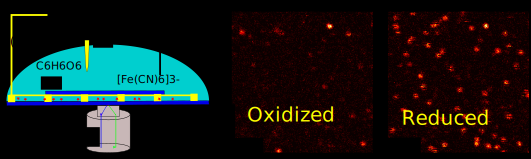
\includegraphics[width=\textwidth]{Scheme_1_setup.eps}
	\caption{The schematic of the confocal and electrochemical setup. \textbf{(1)} Objective through which light is irradiated on and collected from the sample. \textbf{(2)} The functionalized sample slide with on top the platinum grid and another small glass slide to press the grid on the sample slide, resulting in small confined volumes in the order of nanoliters. \textbf{(3)} The electron mediator solution containing of $200~$\uM~ferricyanide, $100~$\uM~ascorbate in PBS (pH 7.4) buffer with a total volume of 4 mL. \textbf{(4)} The working electrode (platinum wire) that is in contact with the platinum grid (yellow blocks). \textbf{(5)} The saturated calomel reference electrode. \textbf{(6)} The platinum wire (not touching the grid) as counter electrode. \textbf{(7)} The potentiostat (Model 800B Series Electrochemical Detector, CH Instruments) to which the electrodes are connected. \textbf{(8, 9)} Top view of the sample slide. The two images are showing the labeled Cu-Azurin reduced(right, brighter) and oxidized(left, dimmer) states.}
  	\label{sch:setup}
\end{scheme}
%%%%%%---------------------RESULTS and DISCUSSION-----------------------%%%%%%%%%
\section{Results and discussion\label{sec:results}}
\subsection{Time traces at different potentials}
Active Cu-azurin molecules were identified from their fluorescence intensity images at the oxidizing ($200~mV$) and reducing conditions($0~mV$). In reducing conditions, the image contains many bright spots corresponding to Cu(I)-azurin-ATTO655 and more than $90~\%$ of the molecules are turned off in oxidizing conditions (Scheme-\ref{sch:setup}(8)). The azurins on each sample slide showed active switching during the course of the experiment (up to two days) without any noticeable degradation. A set of active azurins were marked for recording and time traces at different potentials (between $100~mV$ and $-100~mV$) were measured on the \texttt{same molecules} for $30~s$. Many of the labeled proteins bleached within the recording at a few potentials, but more than $50~$\% of the labeled-azurin survived at least five measurements ($150~s$ total) at different potentials. Longer measurements were possible thanks to the scavenging of oxygen in the solution. Before recording the time trace, the solution was exposed to a negative potential for at least $1~$hour. Ascorbate is known to  scavenge oxygen\cite{dave1997effectiveness} and get oxidized. The oxidized ascorbate is then reduced by the electrode and is again available to scavenge other oxygen molecules. In addition to the absence of oxygen, the ROXS mechanism was also in play.\cite{cordes2009on} The reduction and oxidation of Cu-azurin made the dye switch on and off, hence the fluorescent dye spent less time in the bright state where it is more prone to bleach. This allowed the measurement of fluorescence time traces for more than $1000~s$.\\
%---time trace
\begin{figure}
	\centering
	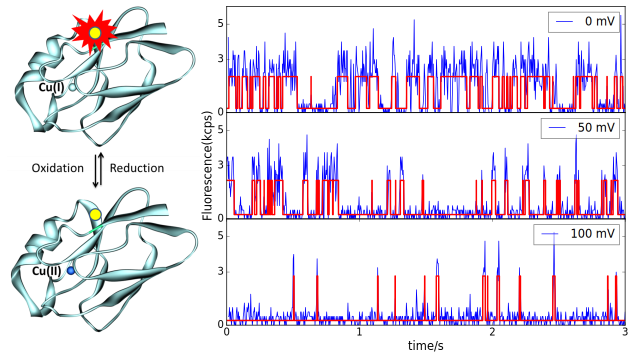
\includegraphics[width=\textwidth]{Figure_1_timetrace_CuAzu.eps}
	\caption{Time traces of Cu-azurin labeled with ATTO655 at different potentials (0, 50 and 100~mV with respect to SCE). The structure of the protein with properly positioned dye can be seen in the schematic picture in the left. In the Cu(II) state (shown as blue dot in the protein structure), the dye is non fluorescent because of FRET and in the Cu(I) state (shown as as a gray dot), the dye is fluorescent. Notice the amount of time the protein spends in the bright and the dark state at different potentials. At lower potentials (e.g 0 mV) the protein is bright most of the time because of the higher concentration of reductant.}
	\label{fig:timetrace}
\end{figure}
Figure-\ref{fig:timetrace} shows time traces of a single Cu-azurin-ATTO655 molecule at three different potentials. The intensity changes from bright to dark and vise versa over time(Figure \ref{fig:timetrace}). The dark state is due to the FRET from the dye to the Cu(II) absorption center\cite{kuznetsova2006a}. Bulk measurements of the fluorescence intensity at completely oxidizing and completely reducing condition shows $90~$\% switching ratio (Figure S\ref{SIfig: switching}) for the lysine-122 labeled Cu-azurin-ATTO655.\cite{nicolardi2012topdown} Also single-molecule measurement (Figure S\ref{SIfig: lifetime}) at a higher laser power $0.7~\uW$ show more than $90~\%$ switching, which is consistent with the bulk measurements. The intensity of Cu(II)-state is lower than the intensity of Cu(I)-state, but higher than the background (bleached state). Also the Cu(II)-state has a shorter lifetime ($0.3~\ns$ than Cu(I)-state ($1.9~\ns$), but longer than the instrument response function ($0.1~\ns$). Both intensity and life time information confirm that the dim-state is FRET quenched. The high FRET efficiency is due to the small distance of the dye to the absorption center. This clear distinction between the on and off state was very important for the low laser power and lower signal measurements. At higher potential ($100~mV$), the protein spends most of the time in dark state and as the potential is lowered, the molecule spends more and more time in the bright state. As we lower the potential, the concentration of the reductant increases, keeping the protein in Cu(I)-state for a longer time. A control study with Zn-azurin-ATTO655 (Figure S\ref{SIfig:tracecomparision} and Figure S\ref{SIfig:fcscomparision}) shows that the dye itself blinks below $40~mV$ due to photo-excited electron transfer. Zinc does not absorb light in the red and does not switch its oxidation state. To simplify the analysis, therefore only potentials above $40~mV$ were considered for the Cu-azurin-ATTO655 study.\\
%Midpoint histogram
\subsection{Midpoint potential of single-azurins}
\begin{figure}
	\centering
	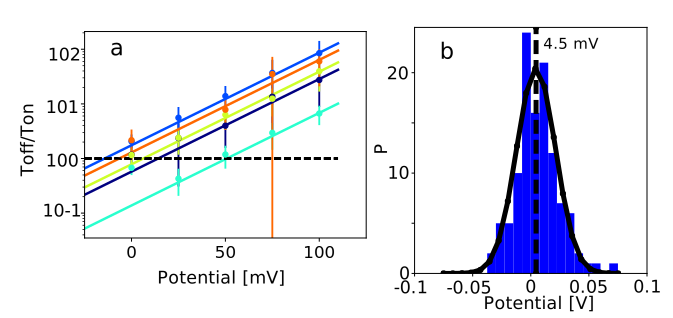
\includegraphics[width=\textwidth]{Figure_2_midpoint.eps}
	\caption{Ratio between on and off time as a function of applied potential for the same single-molecule. Different color represents different single-molecules. And the line connecting the data points is the Nernst fit for all the data points above 25 mV. The plot in the right is the histogram of midpoint potentials for $132$ molecules with a Gaussian fit with a center value of 4.5 mV with respect to calomel electrode.}
	\label{fig:midpoint}
\end{figure}
Figure \ref{fig:midpoint}a shows the ratio between the average off-time ($\me{t}_{off}$) and average on-time($\me{t}_{on}$) plotted against the applied potential. The relationship of this ratio with the potential is given by the Nernst equation: 
\begin{equation}
	E = E_0 + \frac{k_BT}{n e}\ln\left(\frac{\me{t}_{on}}{\me{t}_{off}}\right)\,
	\label{eq:nernst}
\end{equation}
where $E$ is the applied potential, $E_0$ the mid-point potential, $k_B$ the Boltzmann constant, $T$ the absolute temperature, $n$ the number of electrons involved in the reaction and $e$ the electron charge. The value of $n$ was found to be $1$ from the data analysis when the slope in the Nernst equation is kept as a free parameter (see Figure-S\ref{SIfig:potential_slope}). Each color represents a single-azurin and the solid line connecting the points is the fit with the Nernst equation. Labeled proteins surviving at least three potentials above $40~mV$ were used for the fit. The potential at which the off-on ratio equals $1$ is the midpoint potential. The distribution of midpoint potentials(Figure \ref{fig:midpoint}b) from 132 molecules can be fitted by a Gaussian with a center value of $\left<E_0^{SM}\right>=4.5 \pm 1.2~mV$ and a full width half maximum (fwhm) of $\sigma^{SM}=36 \pm 3~mV$. The midpoint potentials are similar to previously reported values of $6\pm0.6~mV$ with $fwhm=150~mV$ where each $E_0$ was calculated from a cluster of about $1000$ molecules.\cite{davis2006monitoring} Another work reported $E_0 = 16~mV$ with low surface coverage (100s of azurins) with a fwhm of $70~mV$.\cite{salverda2010fluorescent} Recently, for truly single-azurin, a midpoint potential of $E_0=12\pm3$ was reported with fwhm of $92~mV$.\cite{akkilic2014chemically-induced}\\
The small width of the distribution ($36~$mV) of single-azurin midpoint potentials in this work is obtained probably because of the way the proteins are functionalized to the surface. The azurin is attached to a peg-chain with a length of ${\sim}20~\nm$. The peg-chain is attached to the surface through NeutrAvidin. Such functionalization minimizes the interaction of the protein with the surface. In previous experiments, the azurin was either non-specifically attached to the surface or attached through a very short linker (<$1~\nm$). The surface interaction to different hydrophobic and electrostatic patches on the protein can alter the ET functionality of the enzyme.
%====================Many single-molecule on-off histogram and their rates=================
\subsection{Intermediate detection from on-off histogram}
\begin{figure}
	\centering
	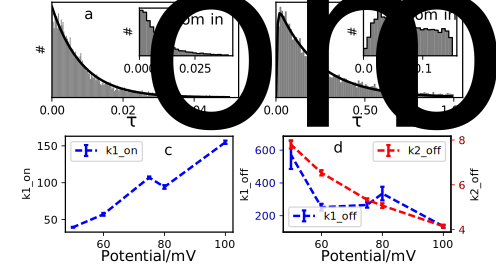
\includegraphics[width=\textwidth]{many_sm_hist.eps}
	\caption{\textbf{Electron transfer rates} The histogram of on-times (a) and off-times (b) of all the single-Cu-azurin-ATTO655 at $100~$mV with their zoomed in part in the inset. Notice the single exponential decay of on-times and the bi-exponential (with rise time) for the off-times. This indicates that  reduction of Cu-azurin occurs through an intermediate step while for oxidation the intermediate state is not observable. The solid line is the corresponding fit to the distribution. (c) The rate constant for oxidation as a function of the potential. (d) The rate constant for reduction as a function of redox potential: blue points correspond to the faster rate constant while the red points represent the slow rate constant.}
	\label{fig:many_sm_hist}
\end{figure}
The on and off times of all the molecules at a certain potential were analyzed together to visualize their overall distribution. Figure \ref{fig:many_sm_hist}(a) shows the histogram of on times at $100~mV$ and the solid line is the fit of a single exponential with a time constant ($k_{on}$) of $155~s^{-1}$. The on-time represents the time the protein spends in the reduced state before getting oxidized according to the following reaction scheme:
\begin{align}
	\ch{!(bright)(Cu(I)Az) + oxd <=>[ $k_1$ ][ $k_{-1}$ ] !(dark)(Cu(II)Az) + red }
	\label{eq:oxidation}
\end{align}
In contrast, the distribution of off-times shows a non-exponential distribution with a rise time Figure \ref{fig:many_sm_hist}(a). The inset clearly shows that the probability of finding protein with very short off-times is relatively small. This distribution can be explained with the Michaelis-Menten mechanism:
\begin{align}
	\ch{!(dark)(Cu(II)Az) + red <=>[ $k_2$ ][ $k_{-2}$ ] !(dark)(Cu(II)Az.red) -> [ k3 ] !(bright)(Cu(I)Az) + oxd}
	\label{eq:reduction}
\end{align}
where $k_2$ is the pseudo-first order rate constant which depends on the concentration of reductant and $k_3$ is the zero order rate constant which should be independent of the concentration of the substrate. When assuming $k_{-2}=0$, the probability distribution of off times is given by\cite{lu1998single-molecule}
\begin{equation}
	P(t_{off}) = \frac{k_2k_3}{k_3-k_2} [exp(-k_2t_{off})-exp(-k_3t_{off})]
	\label{eq:2exp_risetime}
\end{equation}
At $100~$mV, $k_2$ for the reduction is $4.1~s^{-1}$ while $k_3$ is $135~s^{-1}$. The rates were determined at different applied potentials. A linear relationship is observed between the rate of oxidation and the solution potential (Figure \ref{fig:many_sm_hist}(c)). This is in agreement with the first-order kinetic dependent on the concentration of substrate, the concentration of electron mediators vary exponentially with the solution potential. From the slope of the line, a rate constant of $9.4\times10^6~M^{-1}s^{-1}$ for the oxidation is obtained. A similar linear relationship was observed for the $k_2$ of the reduction process as expected with a rate constant of $1.7\times10^5~M^{-1}s^{-1}$.\\
The rate constant ($k_3$) for the second step in the reduction process has a weak dependence on the solution reduction potential(Figure \ref{fig:many_sm_hist}(d, blue)). The value is around $250~s^{-1}$ which is more than an order of magnitude smaller than the rate of intermediate formation.\\
%==================Dynamics: Single-azurin over time===================
\subsection{Dynamics in ET rate}
After looking at many single-azurins, we investigated a single-azurin for long time. Figure \ref{fig:long_azurin_trace} shows the statistics of a single-azurin at $100~mV$ that survived for ${\sim}1250~s$. The distribution of on-and off-times are similar to the distribution of many single-azurin.
%long_azurin_trace
\begin{figure}
	\centering
	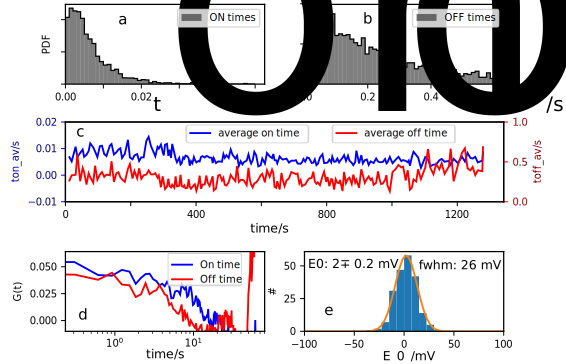
\includegraphics[width=\textwidth]{long_azurin_trace.eps}
	\caption{The histogram of on-times(a) and off-times(b) of a single Cu-Azurin-ATTO655 at $100~mV$ showing rise time similar to many single-azurin distributions. (b) the trace of average on-times (blue) and average off-times (red). The average was calculated every $20$ corresponding on-or off-times. The respective y-scales have the same color as the data points. (d) Autocorrelation of the traces in (c) and the color is matched to the color in the trace. (e) distribution of midpoint potential ($E_0$) calculated from each average on-and off-time from the traces in (c)}
	\label{fig:long_azurin_trace}
\end{figure}

The time trace was divided into small parts and the average was calculated over every $20$ consecutive on-or off-times. Figure \ref{fig:long_azurin_trace}~(c) shows the average on-times (blue) and average off-times (red) as a function of time. Surprisingly, the fluctuations are not simply statistical noise but rather seems to be correlated. The autocorrelations of the average traces show clear decay (Figure \ref{fig:long_azurin_trace}(d)) with decay times around tens of seconds. This means that the rate at which the azurin changes between Cu(II) and Cu(I) state varies over time. Sometimes the frequency at which the state changes is low and sometimes it is high. Such behaviour has been observed previously for other enzymes ($\beta$-galactosidase, flavoenzymes)\cite{lu1998single-molecule,kou2005single-molecule,english2006ever-fluctuating} which is termed as `breathing' in enzymes. A short on-time is followed by a short on-time and a longer on-time is followed by a longer on-time with the memory lasting over a characteristic time scale of tens of seconds. According to the previous report, breathing is a result of slow fluctuations in the structure over time. Azurin is a very small protein ($14~kDa$) and the observation of such variation in ET shows that the ET is very sensitive to the changes in the structure.\\

Also mid-point potentials were calculated from each average on and average off times using the Nernst equation(\ref{eq:nernst}). As both on-and off-times change over time, the midpoint potential too changes over time. The distribution of $E_0$ shows a center value of $2\pm0.2~$mV with a fwhm of $26~$mV. This distribution of midpoint potential of a single-azurin over a long time is similar to the value of $36~$mV obtained from many single-azurins.
%=================CONCLUSION==================
\section{Conclusion}
The results presented here shows how to controllably switch the solution potential and determine the switching ratio of redox active azurin. By introducing non-interacting surface and long linker, very narrow distribution in the midpoint potential obtained. The distribution over many single-azurin was found to be very close to the distribution of a single-azurin over long time. The rate of intermediate formation for the reduction process has been observed conferring to Michaelis-Menten mechanism. The intermediate formation for the oxidation was too fast to be detected with our signal to noise ratio. In principle similar measurement at higher laser power and for many molecule should enable the detection of the intermediate if their is any. For the first time, correlated dynamics observed in the ET of very small azurin whose molecular mechanism still need to be deciphered.
%===============================================================================================
%=================================SUPPORTING INFORMATION========================================
%===============================================================================================
\graphicspath{{chapters/c4_azurin_sm/si/}}
%=====================METHODS AND FIGURES===========================
\section{Supporting Info}
%Peak separation
\begin{figure}
  \centering
  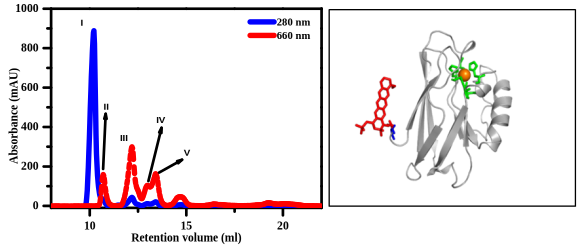
\includegraphics[width=0.8\textwidth]{peak_separation}
  \makeatletter
  \renewcommand{\fnum@figure}{\figurename~S\thefigure}
  \makeatother
  \caption{Peak separation: (a) Elution profile of Cu azurin sample after labeling and removal of free dye.
  \SI{280}{\nm} absorption that tells the presence of protein is shown in blue and \SI{660}{\nm} absrption that tells the presence of  dye is shown in red.
  The protein structure with the dye at Lys corresponding to peak-III is shown in the right. 
  {A proper structure will be replaced}}
  \label{SIfig: peak_sep}
\end{figure}
% \pagebreak
%==================BULK Switching=========================
\paragraph*{Fluorescence switching in bulk} Fluorescence measurements in bulk of different peaks of azurin-ATTO655 sample (Figure S\ref{SIfig: peak_sep}) were carried out to determine the FRET switching ratio.
The measurements were done in Cary Eclipse Spectrometer (Varian Inc. Agilent Technology, USA).
A \SI{50}{\nM} sample was excited with \SI{665}{\nm} and intensity was monitored above \SI{675}{\nm}.
Sodium ascorbate (reductant) and pottasium ferricyanide (oxidant) were added alternatively.
Among all the labeled position, peak-III showed maximum switching ratio and it's intensity change can be seen in Figure S\ref{SIfig: switching}.
Similarly Zn Azurin-ATTO655 showed little or no change in intensity.
\begin{figure}
  \centering
  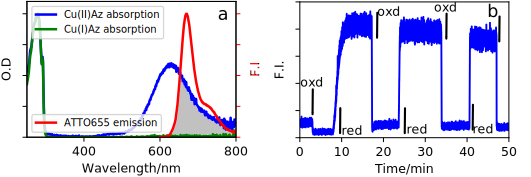
\includegraphics[width=\textwidth]{spectral_overlap_switching}
  \makeatletter
  \renewcommand{\fnum@figure}{\figurename~S\thefigure}
  \makeatother
  \caption{Spectral overlap and Bulk switching: (a) Absorption spectrum of Cu(II)azurin (blue), Cu(I)azurin (blue).
  The emission spectrum of ATTO655 (red) has a good overlap with the absorption of Cu(II)azurin to show high FRET. 
  (b) Fluorescence intensity of \SI{50}{\nM} CuAzurin-ATTO655 shows high intensity in the presence of reductant and low 
  intensity with oxidant.
  The switching ratio comes to be \SI{90}{\percent} satisfying the requirement for single-molecule FRET.}
  \label{SIfig: switching}
\end{figure}
%==================time trace Zn and Cu azurin=================
\begin{figure}
  \centering
  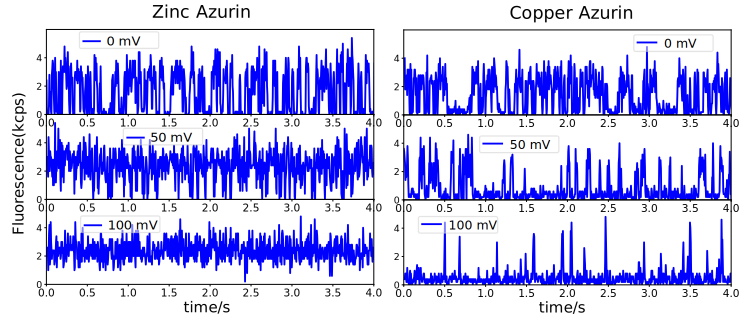
\includegraphics[width=\textwidth,keepaspectratio]{SI_timetrace_Zn_Cu}
  \makeatletter
  \renewcommand{\fnum@figure}{\figurename~S\thefigure}
  \makeatother
  \caption{Time traces of Zn Azurin (left) and of Cu Azurin(right) labeled with ATTO655 at different potential. 
  Above \SI{40}{\mV}, Cu-Azurin show swiching in the intensity due to changes in the oxidation state of the Copper metal center and below \SI{40}{\mV}, triplet blinking contributes to the switching as can be seen in the redox inactive Zn-Azurin.
  To keep the analysis simple, time traces above \SI{40}{\mV} were choosen for Cu azurin}
  \label{SIfig:tracecomparision}
\end{figure}
%===================lifetime and switching ration from time trace================
\begin{figure}
  \centering
  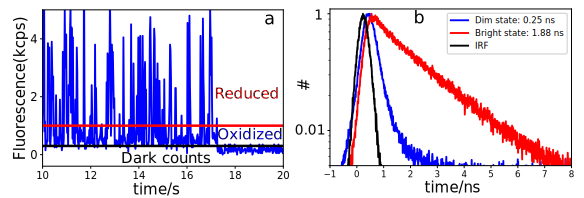
\includegraphics[width=\textwidth]{lifetime}
  \makeatletter
  \renewcommand{\fnum@figure}{\figurename~S\thefigure
}  \makeatother
  \caption{Single-molecule azurin switching and lifetime. (a) Time trace of a single Cu azurin at \SI{50}{\mV} with a binning time of \SI{50}{\ms}.
  Notice the three different labels indicated in the figure. Bright (Cu(I)) state as above the red line, oxidized state is between red and black and Dark counts are below the black line. The fact that the molecule doesn't go to the dark count label before being bleached shows that the transitions are due to Copper oxidation switching rather than triplet blinking of the dye.
  Once the fluorophore is bleached, no transitions were observavable.
  (b) The lifetime histogram corresponding to bright state (red), oxidized state (blue) and instrument response function (black).
  The lifetime of oxidized state is much shorter than the reduced state due to FRET quenching.}
  \label{SIfig: lifetime}
\end{figure}
%=====================FCS comparision=========================
\begin{figure}
  \centering
  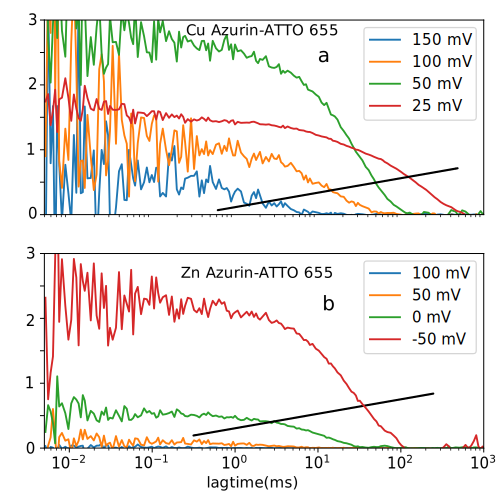
\includegraphics[width=\textwidth]{fcs_comparision}
  \makeatletter
  \renewcommand{\fnum@figure}{\figurename~S\thefigure}
  \makeatother
  \caption{Autocorrelation of time traces of Cuazurin-ATTO655 (a) and Znazurin-ATTO655 at different potential. 
  At lower potential, Cuazurin-ATTO655 has longer correlation time (on time) which shows that the molecule spends more time on the Cu(I) state.
  But below \SI{50}{\mV} the dye (ATTO655) starts to show triplet blinking.
  As potential is lowered the triplet blinking dominates.
  The Cu azurin study is focussed in the safe window of potential more than \SI{40}{\mV} where triplet blinking is absent.}
  \label{SIfig:fcscomparision}
\end{figure}
%===============================Slope: Nernst equation==================================
\begin{figure}
  \centering
  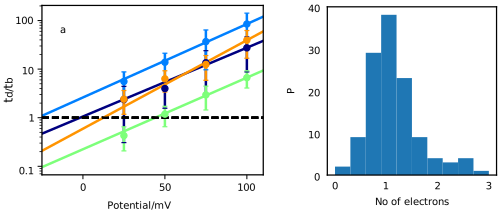
\includegraphics[width=\textwidth,keepaspectratio]{SI_potential_slope}
  \makeatletter
  \renewcommand{\fnum@figure}{\figurename~S\thefigure}
  \makeatother
  \caption{Fitting with Nernst equation with slope as variable parameters for  (a) Cu-Azurin ATTO655. 
  (b) The corresponding histogram of slopes obtained from the fitting shown in the left.T
  he distribution of slope is centered around \SI{59}{\mV} indicating that Cuazurin switching  involves only one electron.}
  \label{SIfig:potential_slope}
\end{figure}
%===================================Rate fit at all potential=============================
\begin{figure}
  \centering
  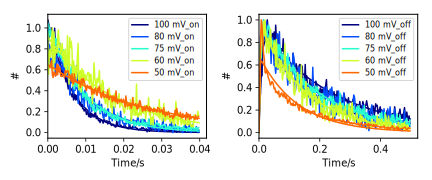
\includegraphics[width=\textwidth]{rate_fit_all_potential}
  \makeatletter
  \renewcommand{\fnum@figure}{\figurename~S\thefigure}
  \makeatother
  \caption{(a) Fitting of $on$ time distribution with monoexponential at different potential.
  (a) Fitting of $off$ time distribution with bi-exponential equation with rise time as shown in the main text at different potential.
  The output rate constants were plotted against potential (see main text)}
  \label{SIfig: rate_fit_all_potential}
\end{figure}
%===================================No of averaging points=================================
\begin{figure}
  \centering
  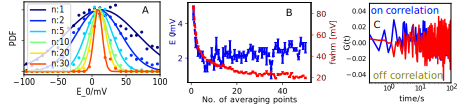
\includegraphics[width=\textwidth]{N_avgpoints_vs_fwhmwidth}
  \makeatletter
  \renewcommand{\fnum@figure}{\figurename~S\thefigure}
  \makeatother
  \caption{\textbf{No correlation dynamics.} Variation of midpoint potential and fwhm with the number of on and off times taken for averaging for the long trace shown in the main text (Figure-\ref{fig:long_azurin_trace}). At around $20~$ events, both $E_0$ and fwhm reaches palteu.
  The averaging of on-time and off-times for correlation and midpoint distribution were done every $20$ events.}
  \label{fig: N_avgpoints_vs_fwhmwidth}
\end{figure}
\paragraph*{}
\begin{figure}
  \centering
  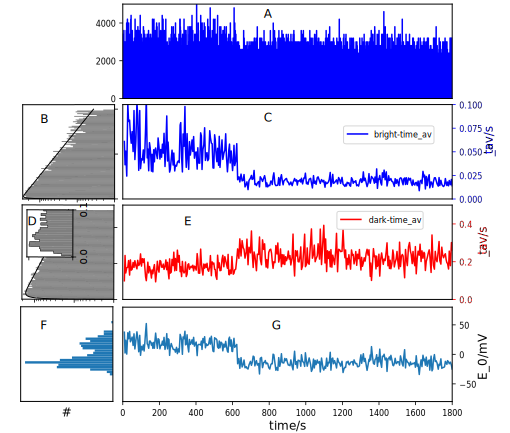
\includegraphics[width=\textwidth]{dynamic_trace_steps}
  \caption{\textbf{Two conformational state dynamics}}
  \label{SIfig:dynamic_trace_steps}
\end{figure}
%============on-off 2D histogram=============
\begin{figure}
  \centering
  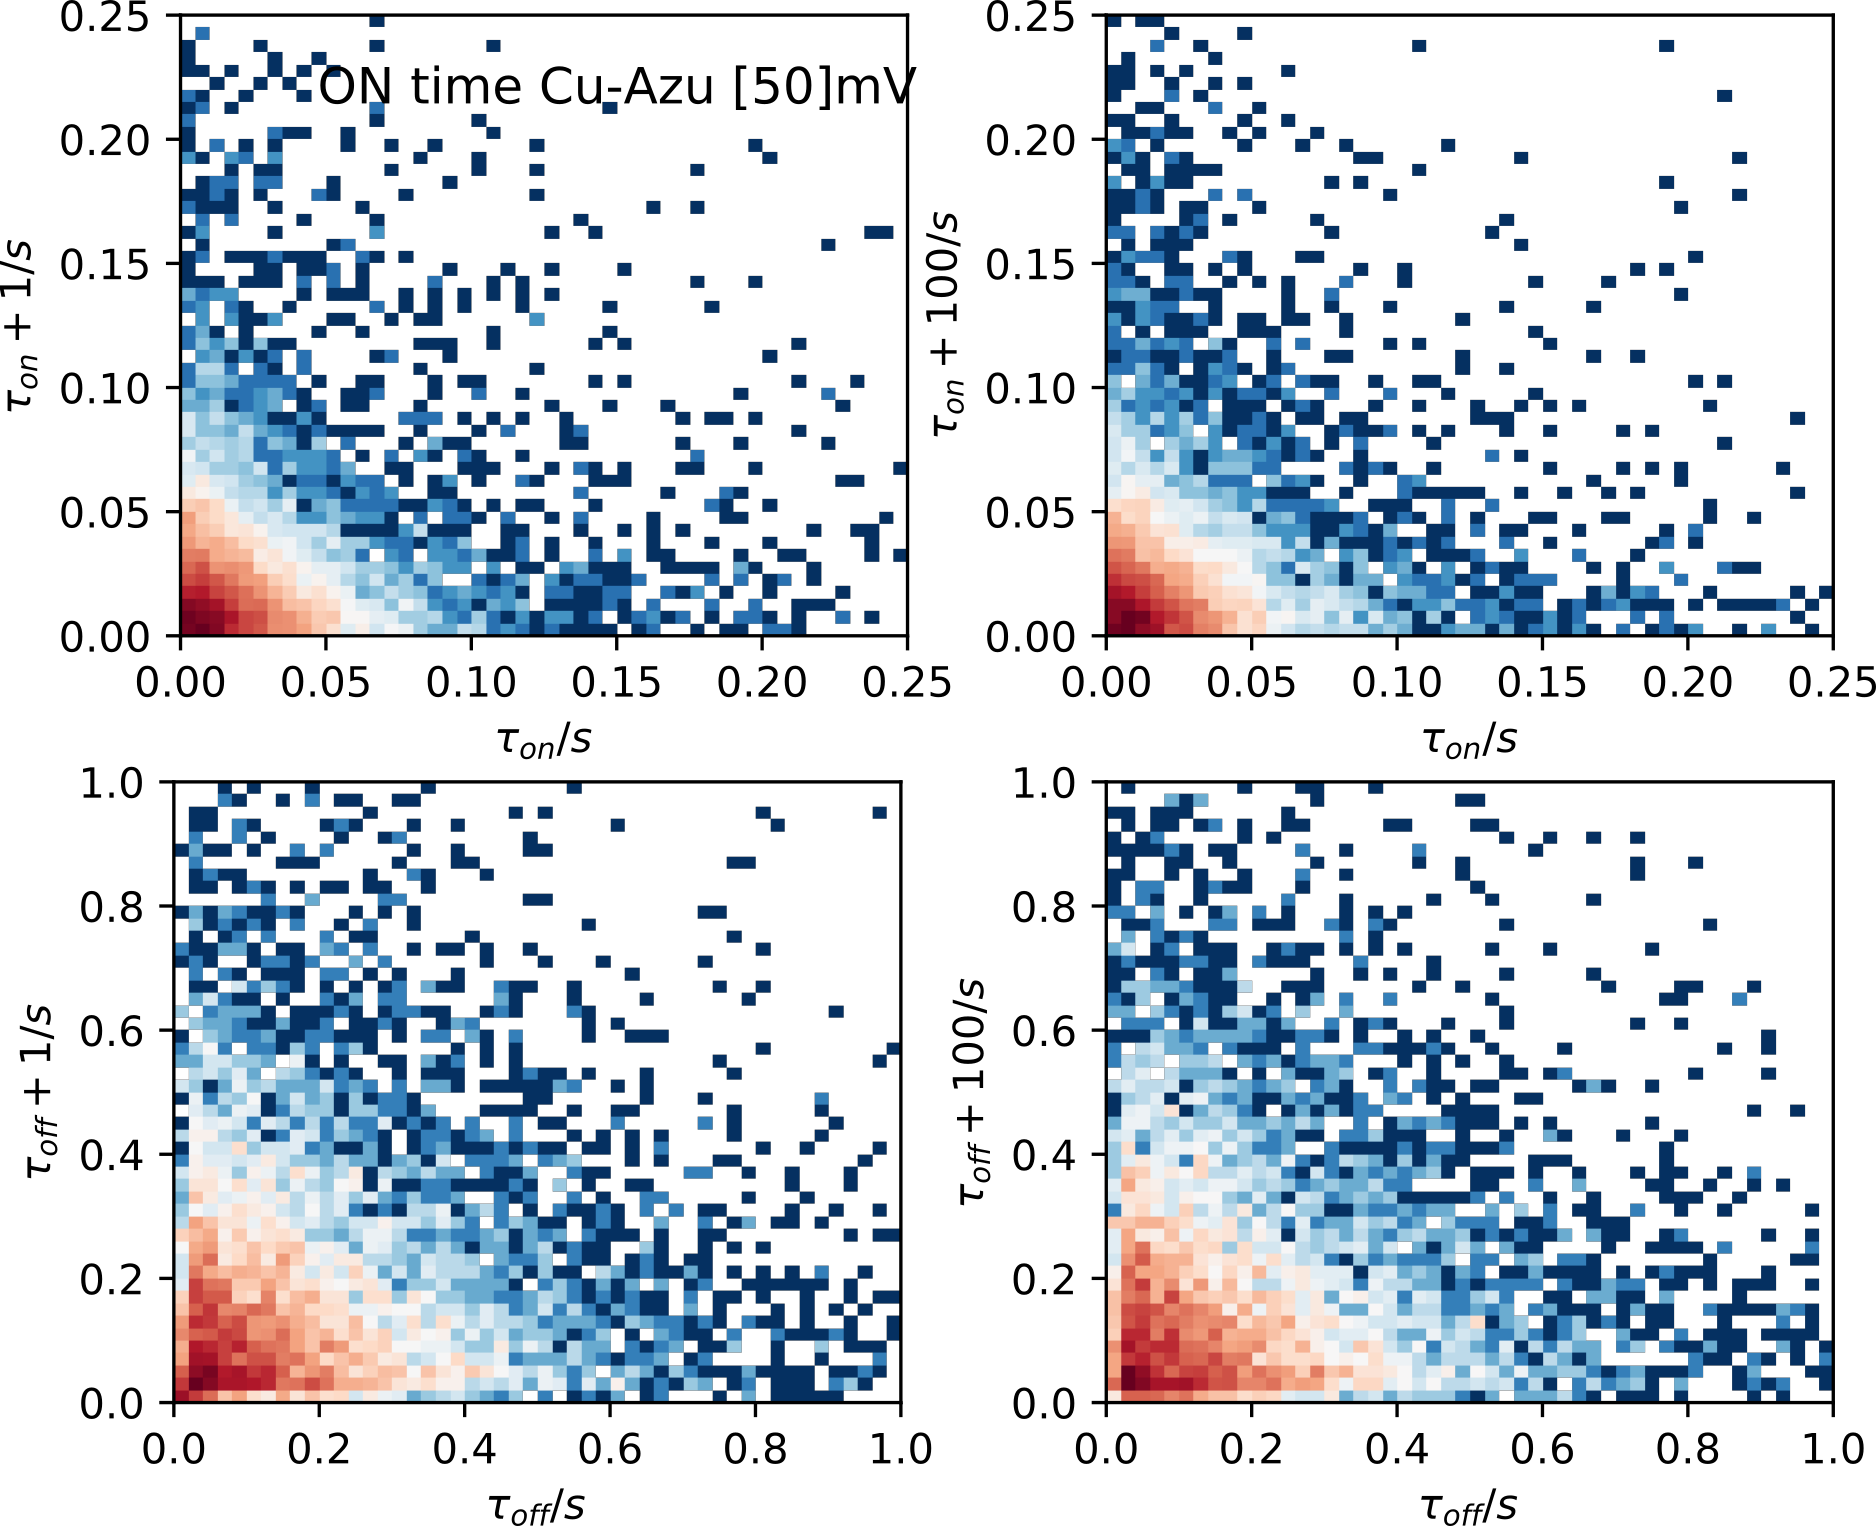
\includegraphics[width=\textwidth]{Figure_4_on_off_2D_100mV}
  \caption{\textbf{2D histogram: Cu-Azurin.}Two-dimensional correlation plot of a single azurin at \SI{50}{\mV} of(a) adjacent waiting time for oxidation ($t_{n}~and~t_{n+1}$) (b) two waiting times at a large separation of 100 ($t_{n}~and~t_{n+100}$) (c) The difference two dimensional histogram of (a) and (b).}
  \label{SIfig:onoff2D}
\end{figure}

\begin{figure}
  \centering
  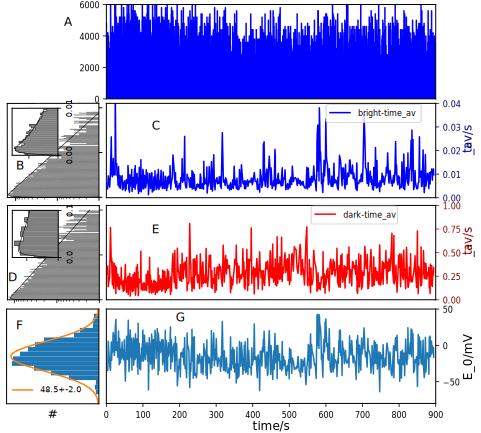
\includegraphics[width=\textwidth]{dynamic_Point_20_75mV_S105}
  \caption{\textbf{dynamic Point 20 75mV S105}}
  \label{SIfig:dynamic_Point_20_75mV_S105}
\end{figure}
\begin{figure}
  \centering
  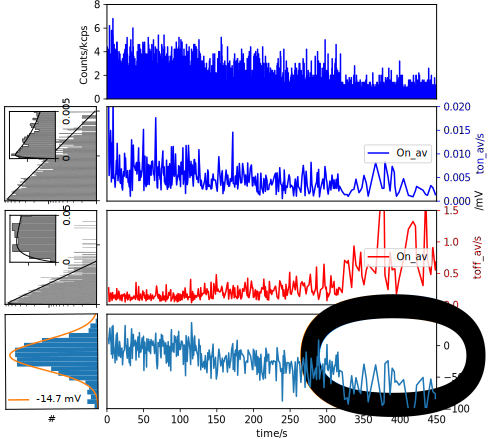
\includegraphics[width=\textwidth]{dynamic_Point_21_75mV_S105}
  \caption{\textbf{dynamic Point 20 75mV S105}}
  \label{SIfig:dynamic_Point_21_75mV_S105}
\end{figure}
\begin{figure}
  \centering
  \includegraphics[width=\textwidth]{Dynamic_corr_many}
  \caption{\textbf{More examples of Dynamic correlation.} 
  }
  \label{SIfig:Dynamic_corr_many}
\end{figure}
\references{chapters/c4_azurin_sm/azurin}